\input ifpdf.sty

\ifpdf
\documentclass[pdftex,beamer,aspectratio=169]{beamer}
\else
\documentclass[xcolor=pst,dvips,beamer]{beamer}
\fi

\usetheme{EnstaB}
\setbeamercovered{transparent}
\useoutertheme{infolines}
\usepackage [frenchb]{babel}
\usepackage[utf8]{inputenc}
\usepackage{verbatim}
\usepackage{pgf,tikz}
\usepackage{amsmath,amssymb,euscript}
\usepackage{eurosym}
\usepackage{float}
\usepackage{mathtools}
\usepackage{algorithm2e}
\usepackage{subcaption}
\usepackage{multicol}
% \usepackage{algorithmic}



\usenavigationsymbolstemplate{}

% \hypersetup{pdftitle={IAMOOC},
%             pdfsubject={Docking project},
%             pdfauthor={Olivier Reynet <olivier.reynet at ensta-bretagne.fr>},
%             pdfkeywords={Interval Analysis, Set Inversion, Contractors},
%             %pdfpagemode={FullScreen}
% }

\usepackage{multicol}
\unitlength 1cm
% ensembles
\RequirePackage{dsfont}
\def\nbR{\mathds{R}}
\def\nbN{\mathds{N}}
\def\nbQ{\mathds{Q}}
\def\nbZ{\mathds{Z}}


\theoremstyle{definition}
\newtheorem{defi}{Définition}
\theoremstyle{example}
\newtheorem{remarque}{Remarque}
\newtheorem{remarques}{Remarques}
\newtheorem{exemple}{Exemple}
\theoremstyle{plain}
\newtheorem{theoreme}{Théorème}
\newtheorem{propriete}{Propriétés}
\newtheorem{lemme}{Lemme}
\newtheorem{corollaire}{Corollaire}

\title[Docking]{Docking autonome pour USV}
\author[]{Théo Massa, Kevin Ren, Guillaume Garde, Hugo Hofmann}
\date{8 Mars 2024}
\titlegraphic{
\includegraphics[width=3cm]{logo_ensta.jpg} 
\includegraphics[width=3cm]{logo-lab-sticc2.png} 
\includegraphics[width=3cm]{logo_ubs_transparent.png} 
}

\institute{ENSTA Bretagne-Lab STICC-Université Bretagne Sud}

\newcommand{\ct}{\cos(\theta)}
\newcommand{\st}{\sin(\theta)}
\usepackage{amssymb} % for \mathbb


\graphicspath{{../Rapport/imgs/}}


\AtBeginSection[]
{
    \begin{frame}
    \frametitle{Plan}
    \tableofcontents[currentsection,currentsubsection]
    \end{frame}
}
%%% Chaque section commence par une slide de rappel de la partie actuelle
%% Il y a des exemples de slides dans les fichiers .tex/.pdf "exemple"

\begin{document}

\frame{\titlepage}

\begin{frame}[allowframebreaks]
  \tableofcontents
\end{frame}

\section{Introduction} 
\begin{frame}{Introduction}
  \begin{minipage}{0.6\textwidth}
    \begin{figure}
      \centering
      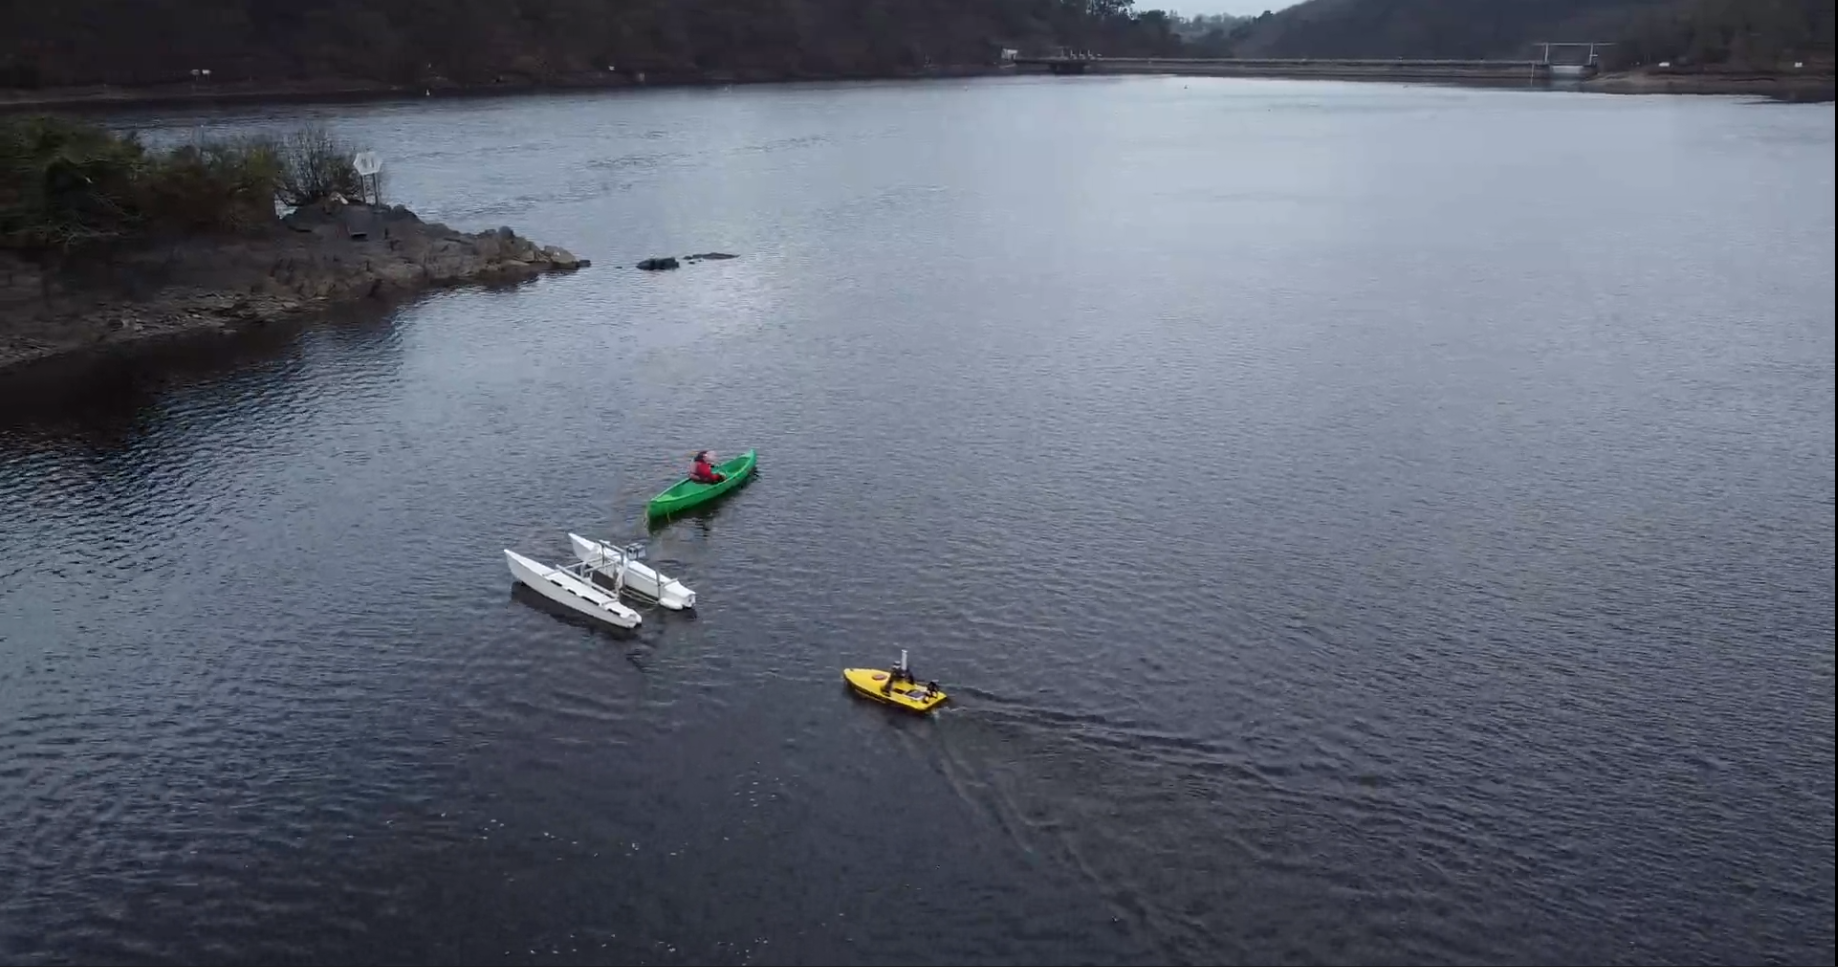
\includegraphics[width=0.9\textwidth]{img_lac.png}
    \end{figure}
  \end{minipage}\hfill
  \begin{minipage}{0.39\textwidth}
    \begin{itemize}
      \item Créer une solution de docking autonome
      \item Véhicule de surface
      \item Utilisation de capteurs basiques
      \item Création d'un système physique pour le dock
    \end{itemize}
  \end{minipage}
\end{frame}

\section{Conception du dock}

\subsection{Base RTK}
\begin{frame}[fragile]{Base RTK}
  Test
\end{frame}

\subsection{Mise en place du dock}

\begin{frame}[fragile]{Mise en place du dock}
  % \vspace{2cm}
  \begin{minipage}{0.5\textwidth}
    \begin{itemize}
      \item Boîte étanche
      \item IMU en dehors (perturbations électromagnétiques)
    \end{itemize}
  \end{minipage}
  \begin{minipage}{0.49\textwidth}
    \begin{figure}[H]
      \centering
      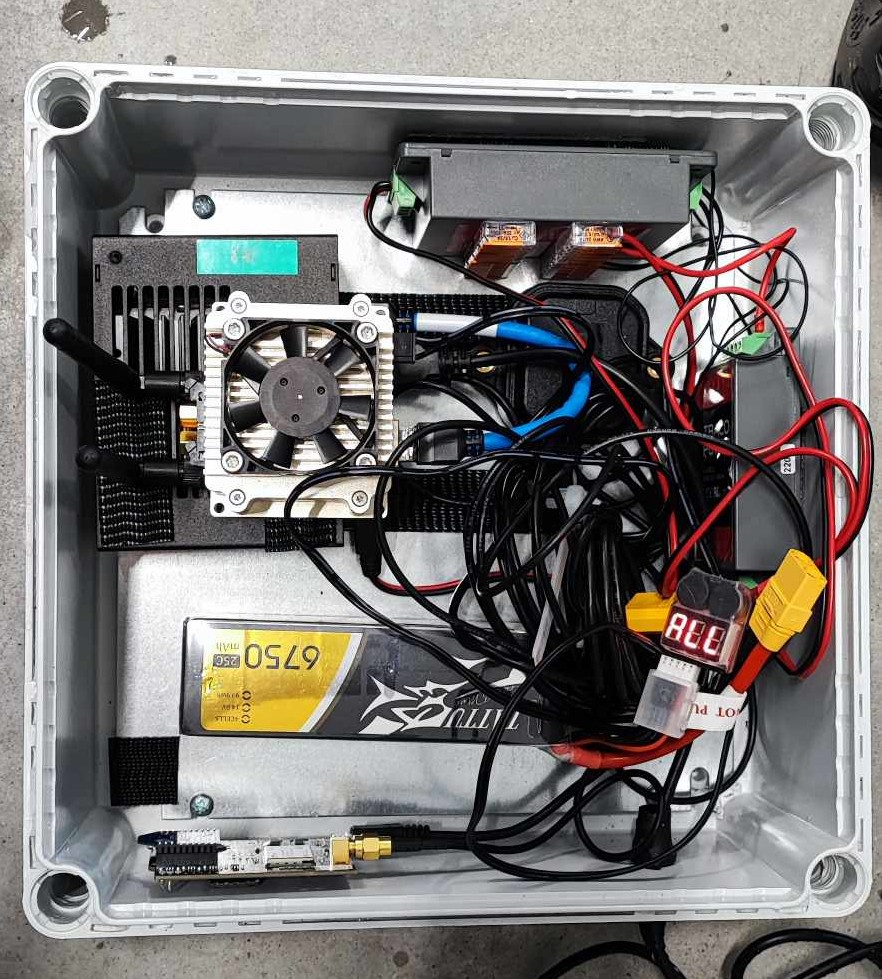
\includegraphics[width=0.7\textwidth]{dock_box_inside.jpg}
      \caption{Mise en place du dock}
    \end{figure}
  \end{minipage}
\end{frame}

\begin{frame}[fragile]{Dock entier}
  \begin{figure}
    \centering
    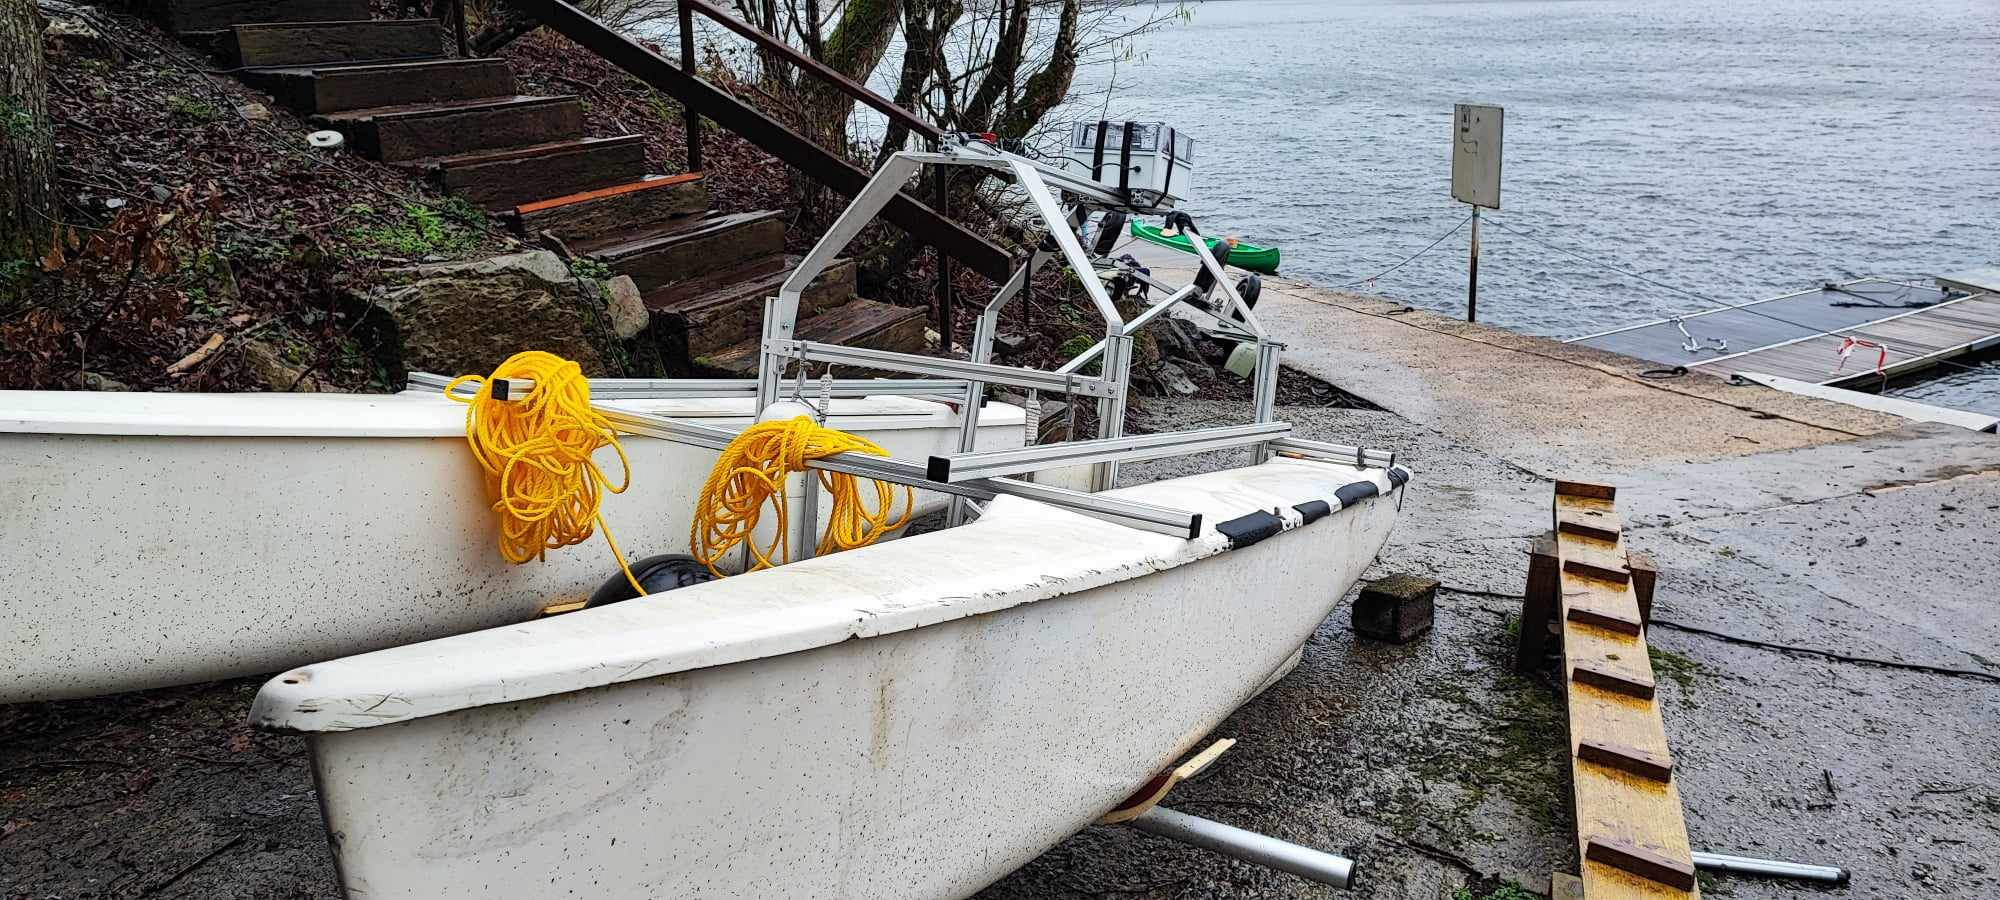
\includegraphics[width=0.9\textwidth]{dock.jpg}
  \end{figure}
\end{frame}

\subsection{Communication}

\begin{frame}[fragile]{Communication avec le reste du système}
  \centering
  \begin{minipage}{0.3\textwidth}
    \begin{exampleblock}{Avantages}
      \begin{itemize}
        \item Format léger
        \item Compatible peu importe les versions de ROS
      \end{itemize}
    \end{exampleblock}
  \end{minipage}
  \begin{minipage}{0.69\textwidth}
    \verb|${latitude},{longitude};{roll},{pitch},{yaw}|
  
    \begin{figure}[H]
      \centering
      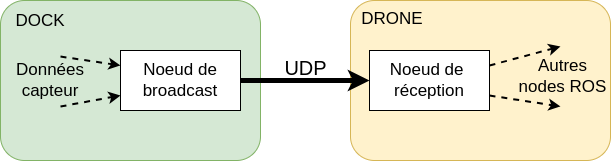
\includegraphics[width=0.9\textwidth]{UDP_connexion.png}
      \caption{La communication dock $\rightarrow$ drone}
  \end{figure}

  \end{minipage}
\end{frame}

\section{Stratégie d'approche de docking}
\subsection{Filtre de Kalman}
\begin{frame}[fragile]{Filtre de Kalman}
  \begin{minipage}{0.5\textwidth}
    Modèle de Dubins : 
    \begin{itemize}
      \item Vecteur d'état $\textbf{x}=(x, y, z, \psi)^T$
      \item Mesure $\textbf{y}=(x_{GPS}, y_{GPS}, \psi_{GPS/IMU})^T$
    \end{itemize}
  \end{minipage}
  \begin{minipage}{0.49\textwidth}
    \begin{figure}[H]
      \centering
      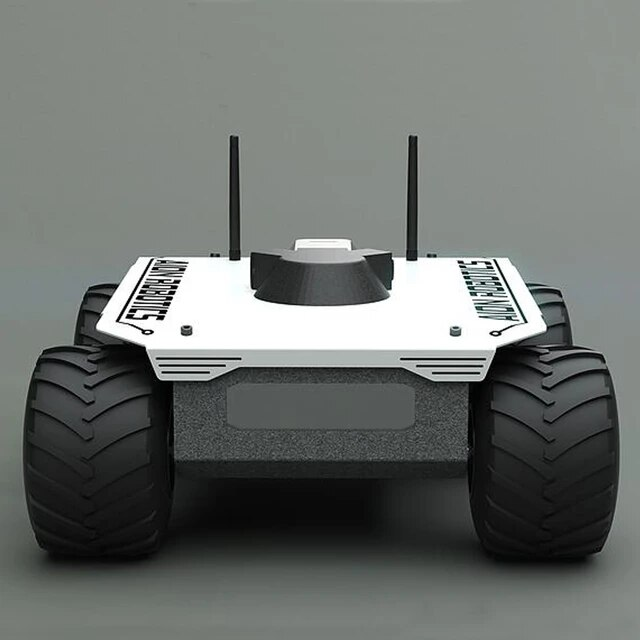
\includegraphics[width=0.7\textwidth]{rover.jpg}
      \caption{Rover}
    \end{figure}
  \end{minipage}
\end{frame}

\begin{frame}[fragile]{Filtre de Kalman}
    \begin{figure}
      \centering
      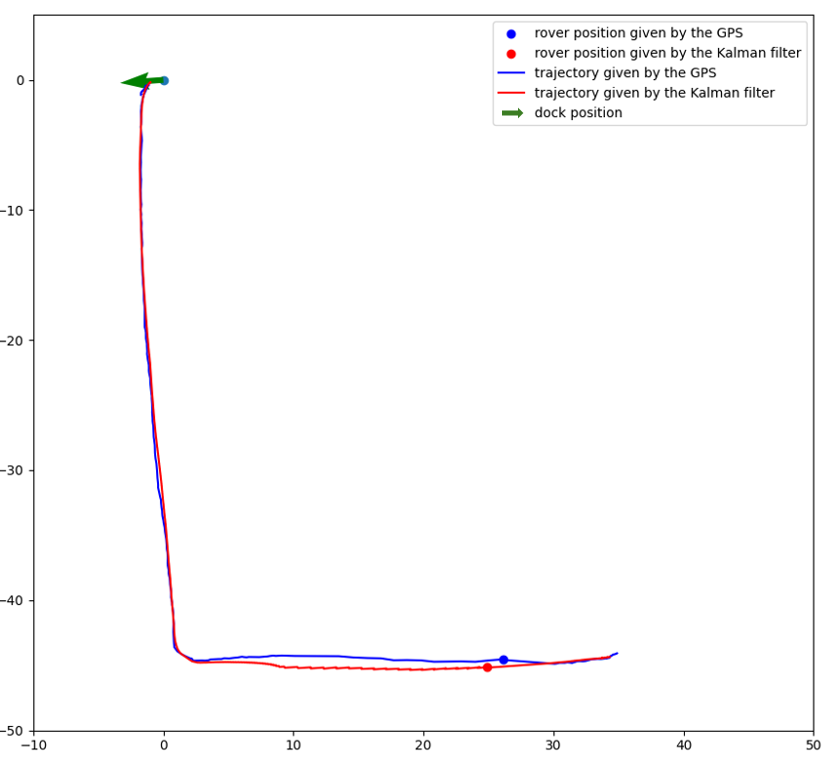
\includegraphics[width=.42\textwidth]{GPSvsKalman.png}
      \caption{Comparatif les données du filtre de Kalman et les données brutes}
      \label{fig:KalmanvsGPS}
    \end{figure}
\end{frame}

\subsection{Guidage par champ de potentiel artificiel}
\begin{frame}[fragile]{Guidage par champ de potentiel artificiel}
  \begin{figure}
  \centering
  \includegraphics[width=12.8cm,height=5.4cm]{RapportGuerlédan-image-1.png}
  \caption{(a) À gauche le robot se trouve dans le demi-plan en face du robot (b) À droite le robot se trouve dans le demi-plan derrière le dock}
\end{figure}

\end{frame}

\begin{frame}[fragile]{Guidage par champ de potentiel artificiel}

\begin{figure}[H]
  \resizebox{0.39\columnwidth}{!}{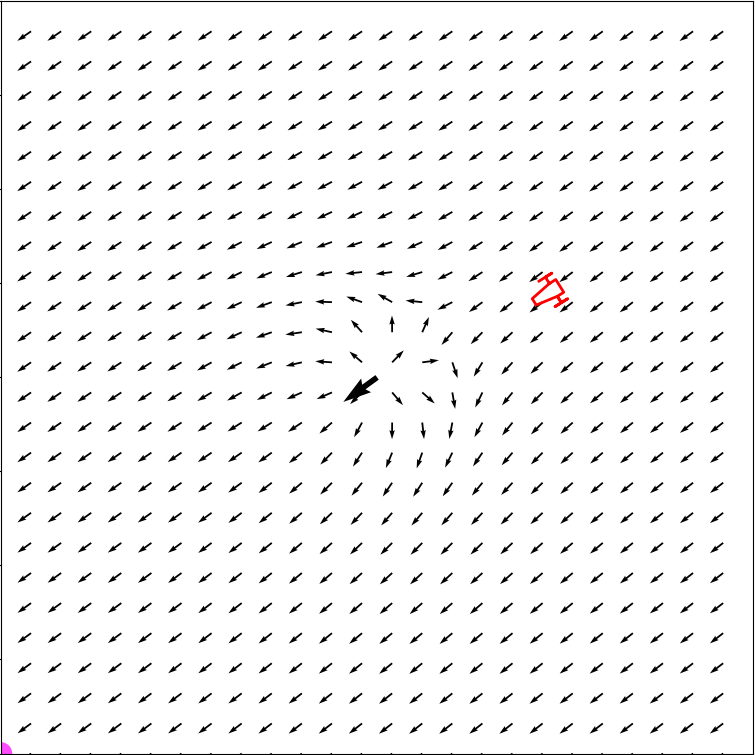
\includegraphics{ScreenshotCase2.png}}\resizebox{0.39\columnwidth}{!}{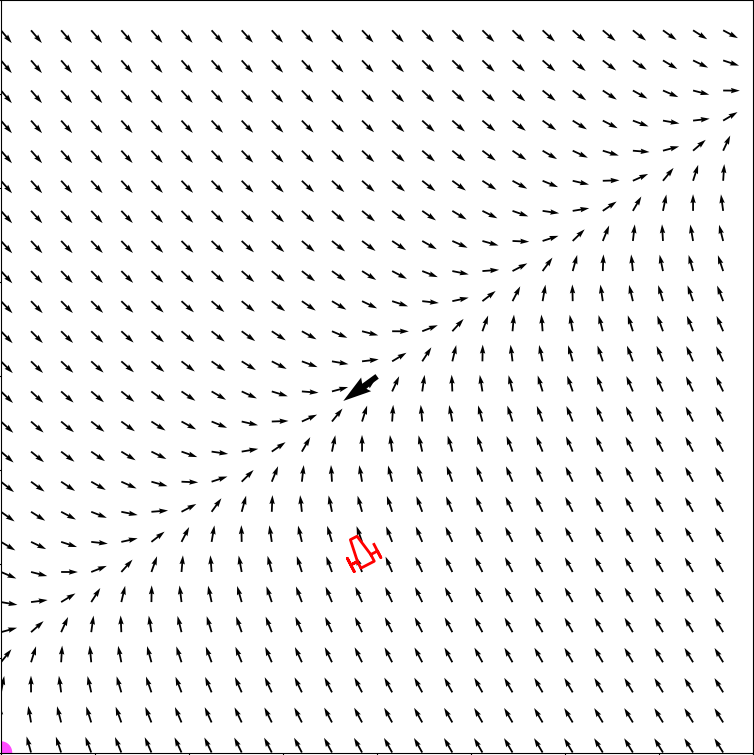
\includegraphics{ScreenshotCase1.png}}
  \caption{(a) Champ de vecteurs dans le premier cas. (b) Champ de vecteurs dans le second cas.}
\end{figure}

\end{frame}

\subsection{Algorithme}
\begin{frame}[fragile]{Algorithme}
  \begin{minipage}{0.5\textwidth}
    Commande en vitesse linéaire et angulaire. \\
    Régulation en cap via un PI. \\ \\
    Instabilité au niveau de la ligne séparatrice, les conditions de transition ont été adaptées : 
    \begin{eqnarray}
        if \ \overrightarrow{M'M} . \overrightarrow{t}<-L \ and \ cas 1 \Rightarrow  \ cas 2 \\
        if \ \overrightarrow{M'M} . \overrightarrow{t}>L \ and \ cas 2 \Rightarrow  \ cas 1
    \end{eqnarray}
  \end{minipage}
  \begin{minipage}{0.49\textwidth}
    \begin{figure}[H]
      \centering
      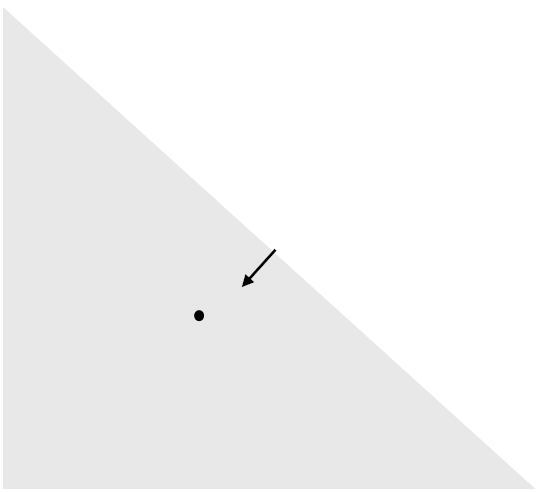
\includegraphics[width=0.7\textwidth]{ligneSep.png}
      \caption{Ligne séparatrice}
    \end{figure}
  \end{minipage}
\end{frame}

\section{Architecture logicielle}
\subsection{ROS}
\begin{frame}[fragile]{ROS}
  \centering
  \begin{minipage}{0.3\textwidth}
    \begin{figure}
      \centering
      
\includegraphics[width=0.9\textwidth]{melodic.png}
      \caption{ROS Melodic}
    \end{figure}
  \end{minipage}\hfill
  \begin{minipage}{0.65\textwidth}
    \begin{figure}
      \centering
      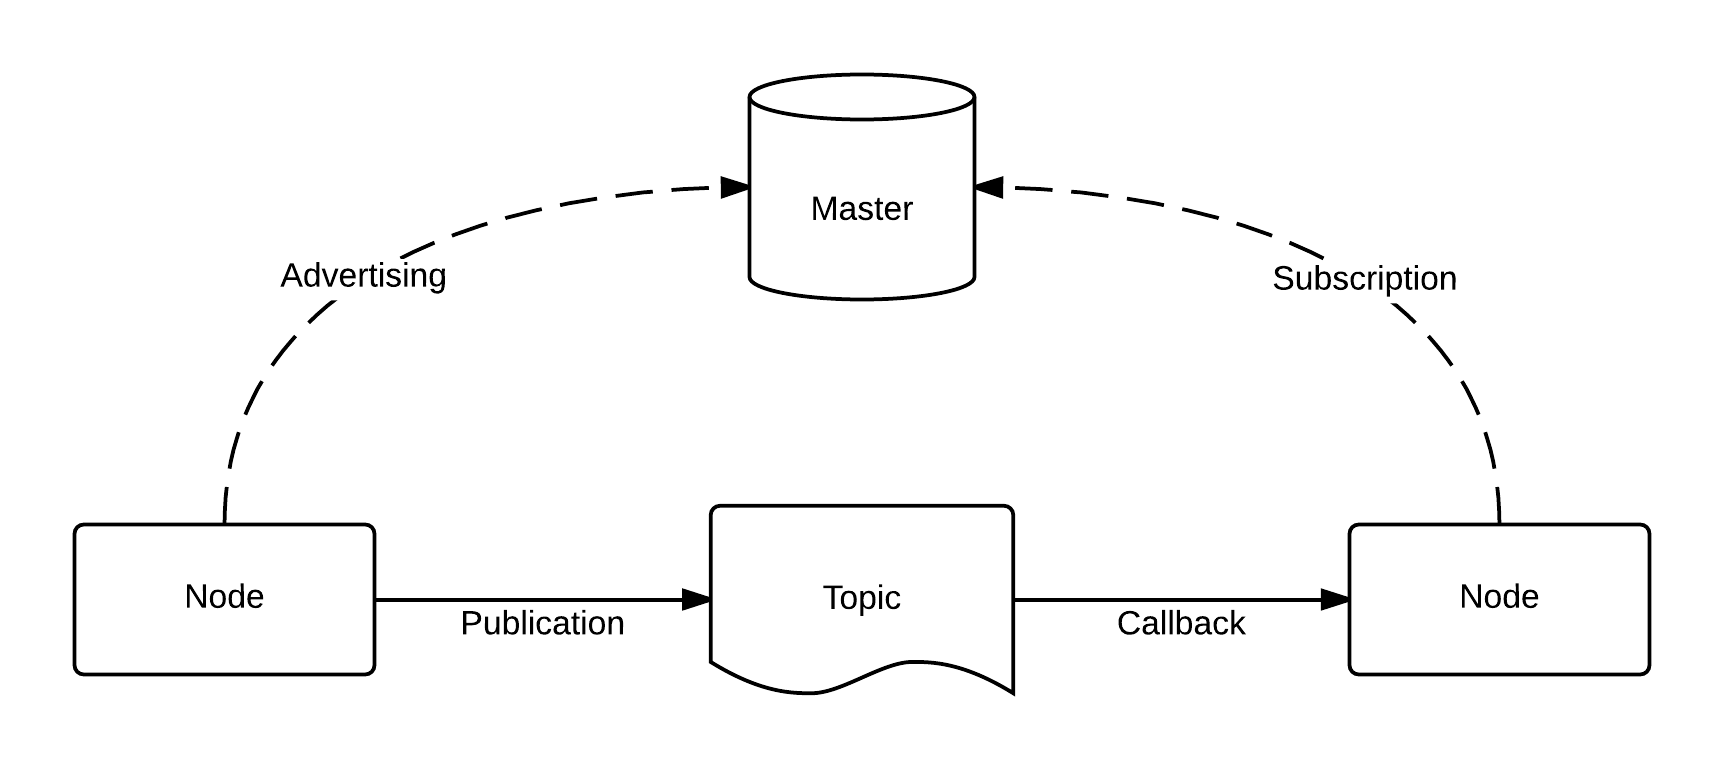
\includegraphics[width=0.8\textwidth]{ROS-master-node-topic.png}
      \caption{Schéma de fonctionnement}

    \begin{exampleblock}{Principe de ROS}
      \begin{itemize}
        \item Middleware commun en robotique
        \item Principe de nodes/topics
      \end{itemize}
    \end{exampleblock}
    \end{figure}
  \end{minipage}
\end{frame}

\subsection{Architecture du projet}

\begin{frame}[fragile]{Architecture du projet}
  \centering
  \begin{minipage}{0.69\textwidth}
    \begin{figure}
      \centering
      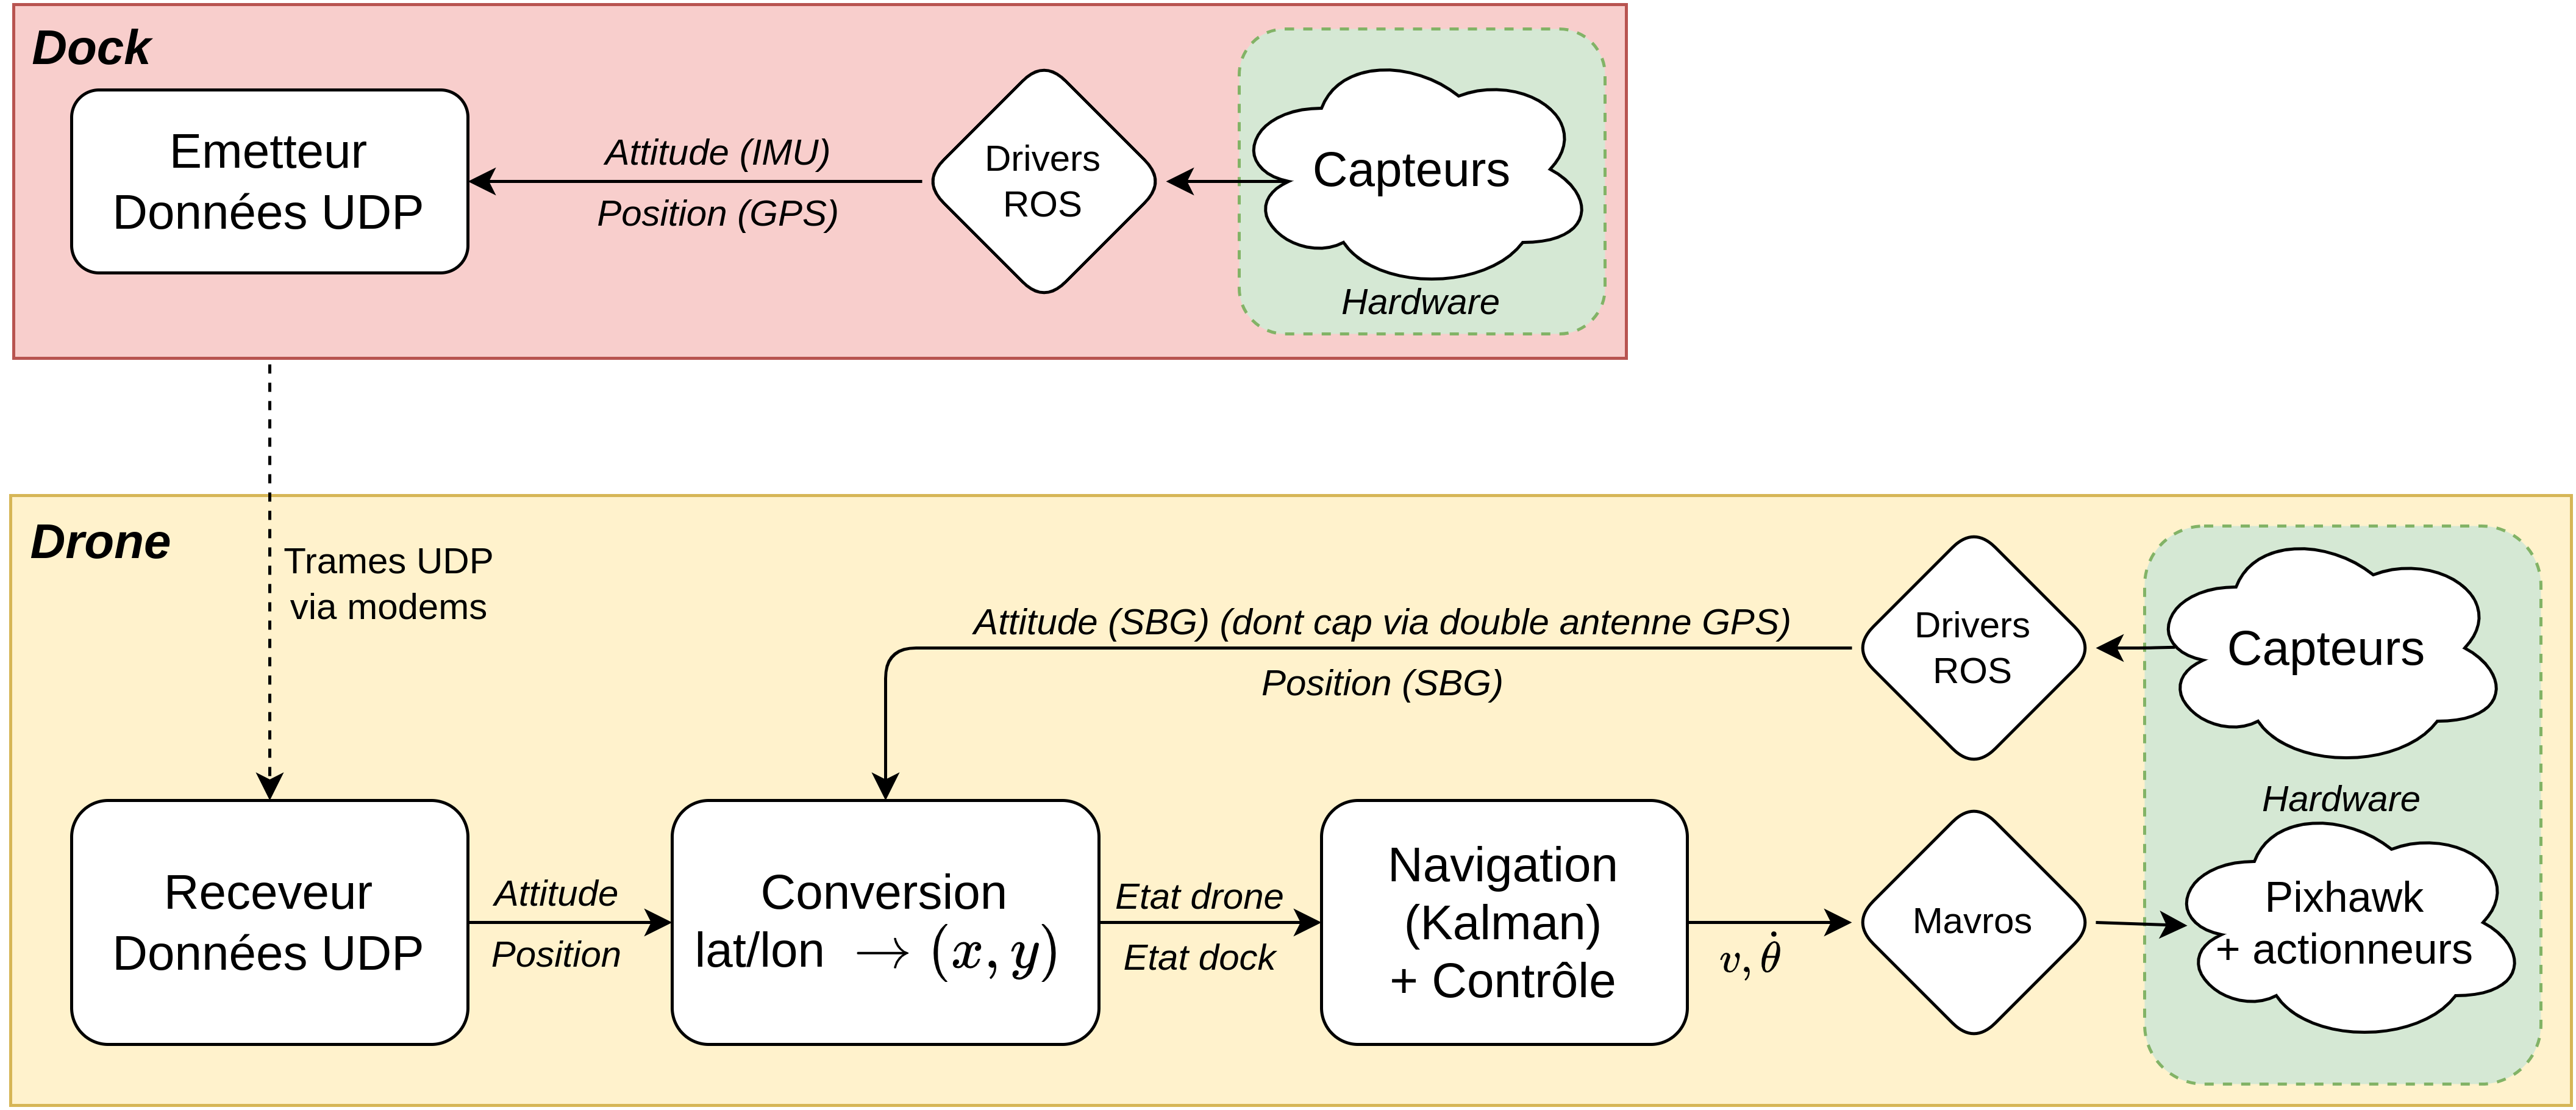
\includegraphics[width=\textwidth]{schema_general.png}
      \caption{Schéma général de l'architecture du projet}
    \end{figure}
  \end{minipage}\hfill
  \begin{minipage}{0.3\textwidth}
    \begin{figure}
      \centering
      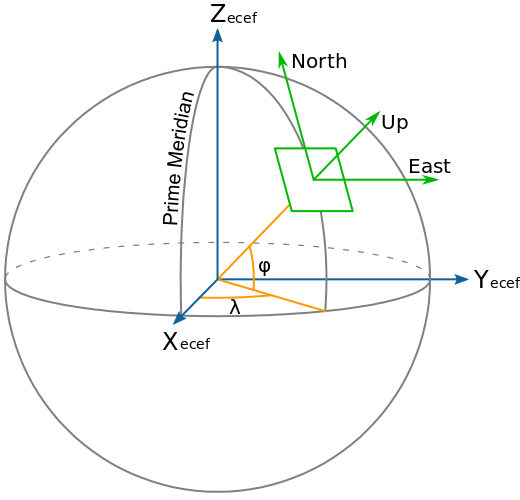
\includegraphics[width=0.9\textwidth]{ENU.png}
      \caption{Repère ENU}
    \end{figure}
  \end{minipage}
\end{frame}

\section{Résultats}

\begin{frame}[fragile]{Résultats}
  \begin{figure}
    \centering
    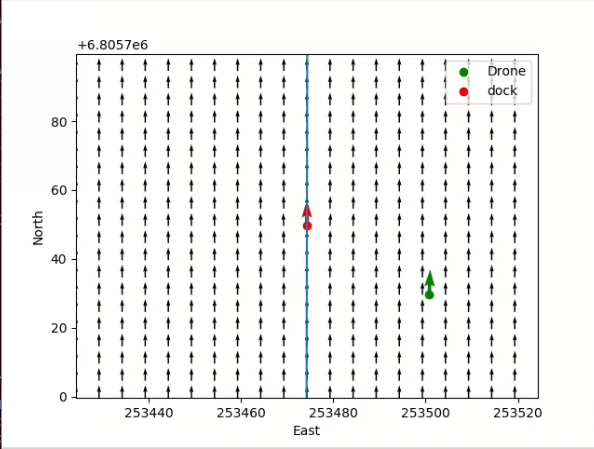
\includegraphics[width=0.3\textwidth]{drone_exp1_1.png}
    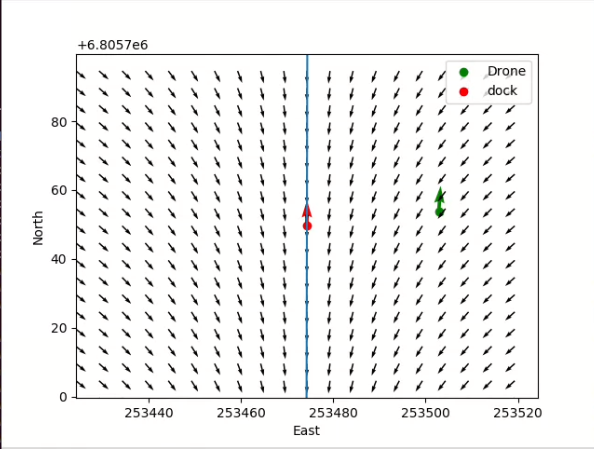
\includegraphics[width=0.3\textwidth]{drone_exp1_2.png}
    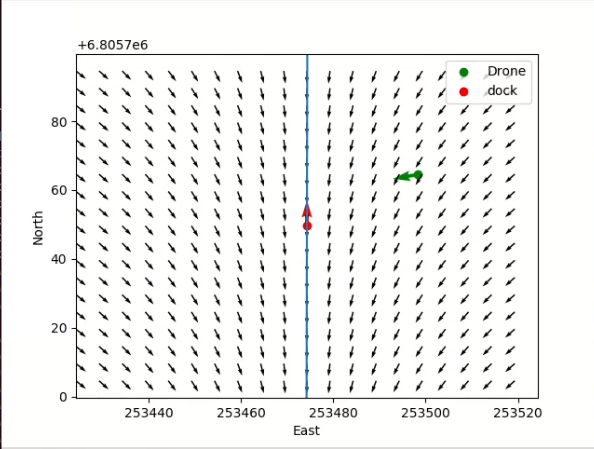
\includegraphics[width=0.3\textwidth]{drone_exp1_3.png}
    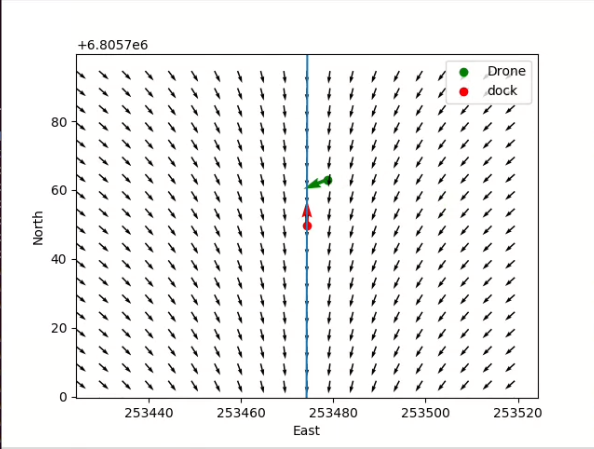
\includegraphics[width=0.3\textwidth]{drone_exp1_4.png}
    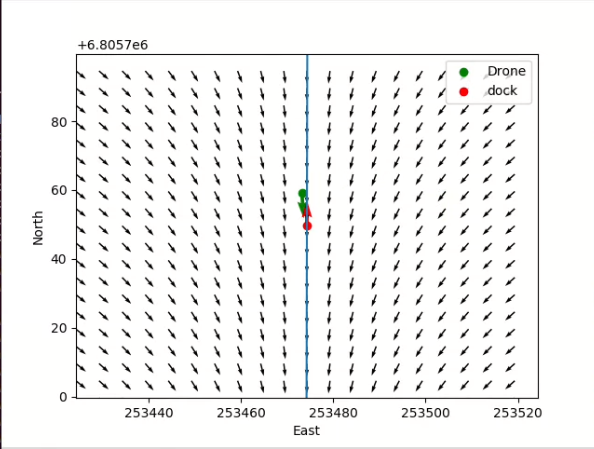
\includegraphics[width=0.3\textwidth]{drone_exp1_5.png}
    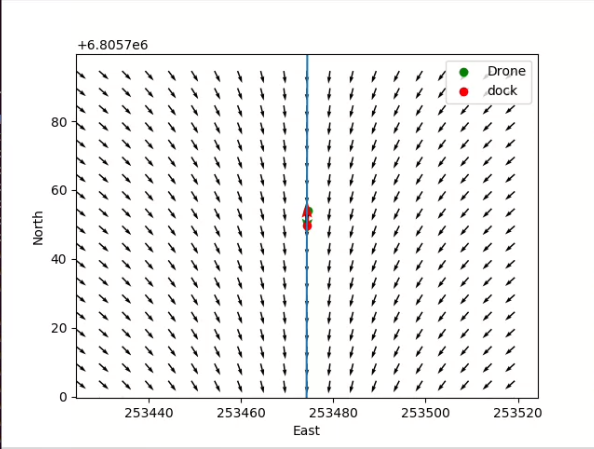
\includegraphics[width=0.3\textwidth]{drone_exp1_6.png}
    \caption*{Algorithme mis en place sur le lac}
    
  \end{figure}
\end{frame}

\begin{frame}[fragile]{Résultats}
  \begin{figure}
    \centering
    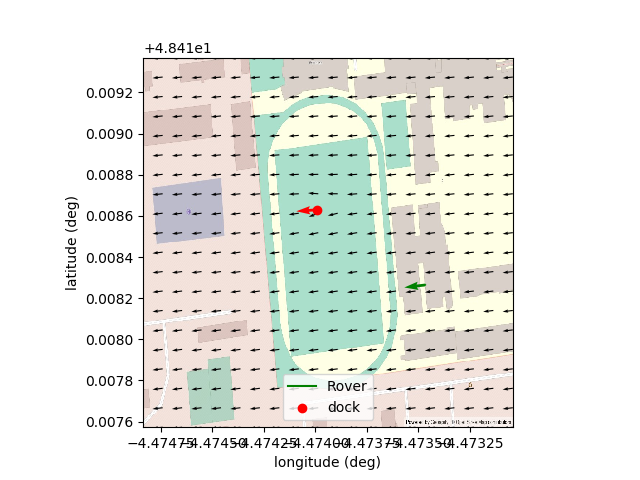
\includegraphics[width=0.49\textwidth]{visu_2.png}
    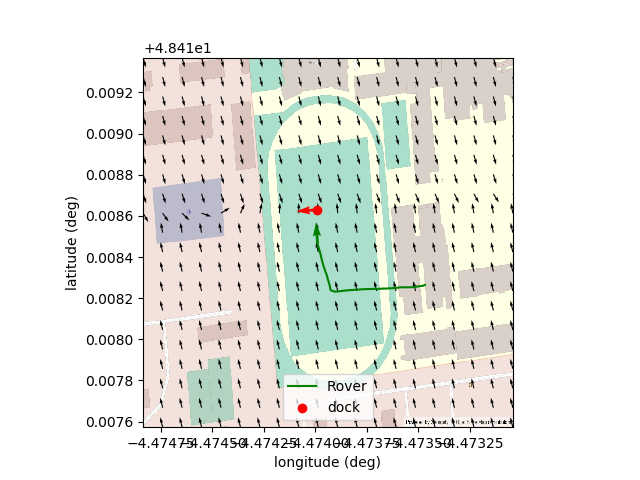
\includegraphics[width=0.49\textwidth]{visu_1.png}
    \caption*{Algorithme mis en place sur le stade avec le rover}
  \end{figure}
\end{frame}

\begin{frame}[fragile]{Conclusion}
  \begin{minipage}{0.49\textwidth}
    Différents points de validation
    \begin{itemize}
      \item Objectif globalement accompli
      \item Navigation et guidage très efficaces
      \item Architecture efficace
    \end{itemize}
  \end{minipage}
  \begin{minipage}{0.49\textwidth}
    Futur du projet
    \begin{itemize}
      \item Calibration correcte du dock
      \item Plus d'essais en lac avec vrai dock
      \item Mise en place de la correction RTK
    \end{itemize}
  \end{minipage}
\end{frame}

\end{document}
